\chapter{Prototype Implementation}
\label{chap:referenceimplementation}

This chapter will discuss how the prototype was designed, implemented and evaluated. \todo{Sections}

\section{System Design}
\label{sec:system_design}

This section will describe the envisioned system for the urban parking availability detection system. The proposed system is a mobile sensing system where sensing vehicles try to detect parking cars while driving through the city. 

- System description (type of sensors, requirements); overall envisioned system of cars detecting free spaces and communicating the information

\subsection{Test Bed Description}
\label{sec:test_bed}

- Testbed description (concrete HW and technical capabilities)

Figure \ref{fig:sensing_car} shows the sensing car and its mounted sensors. 

\begin{figure}
	\centering
	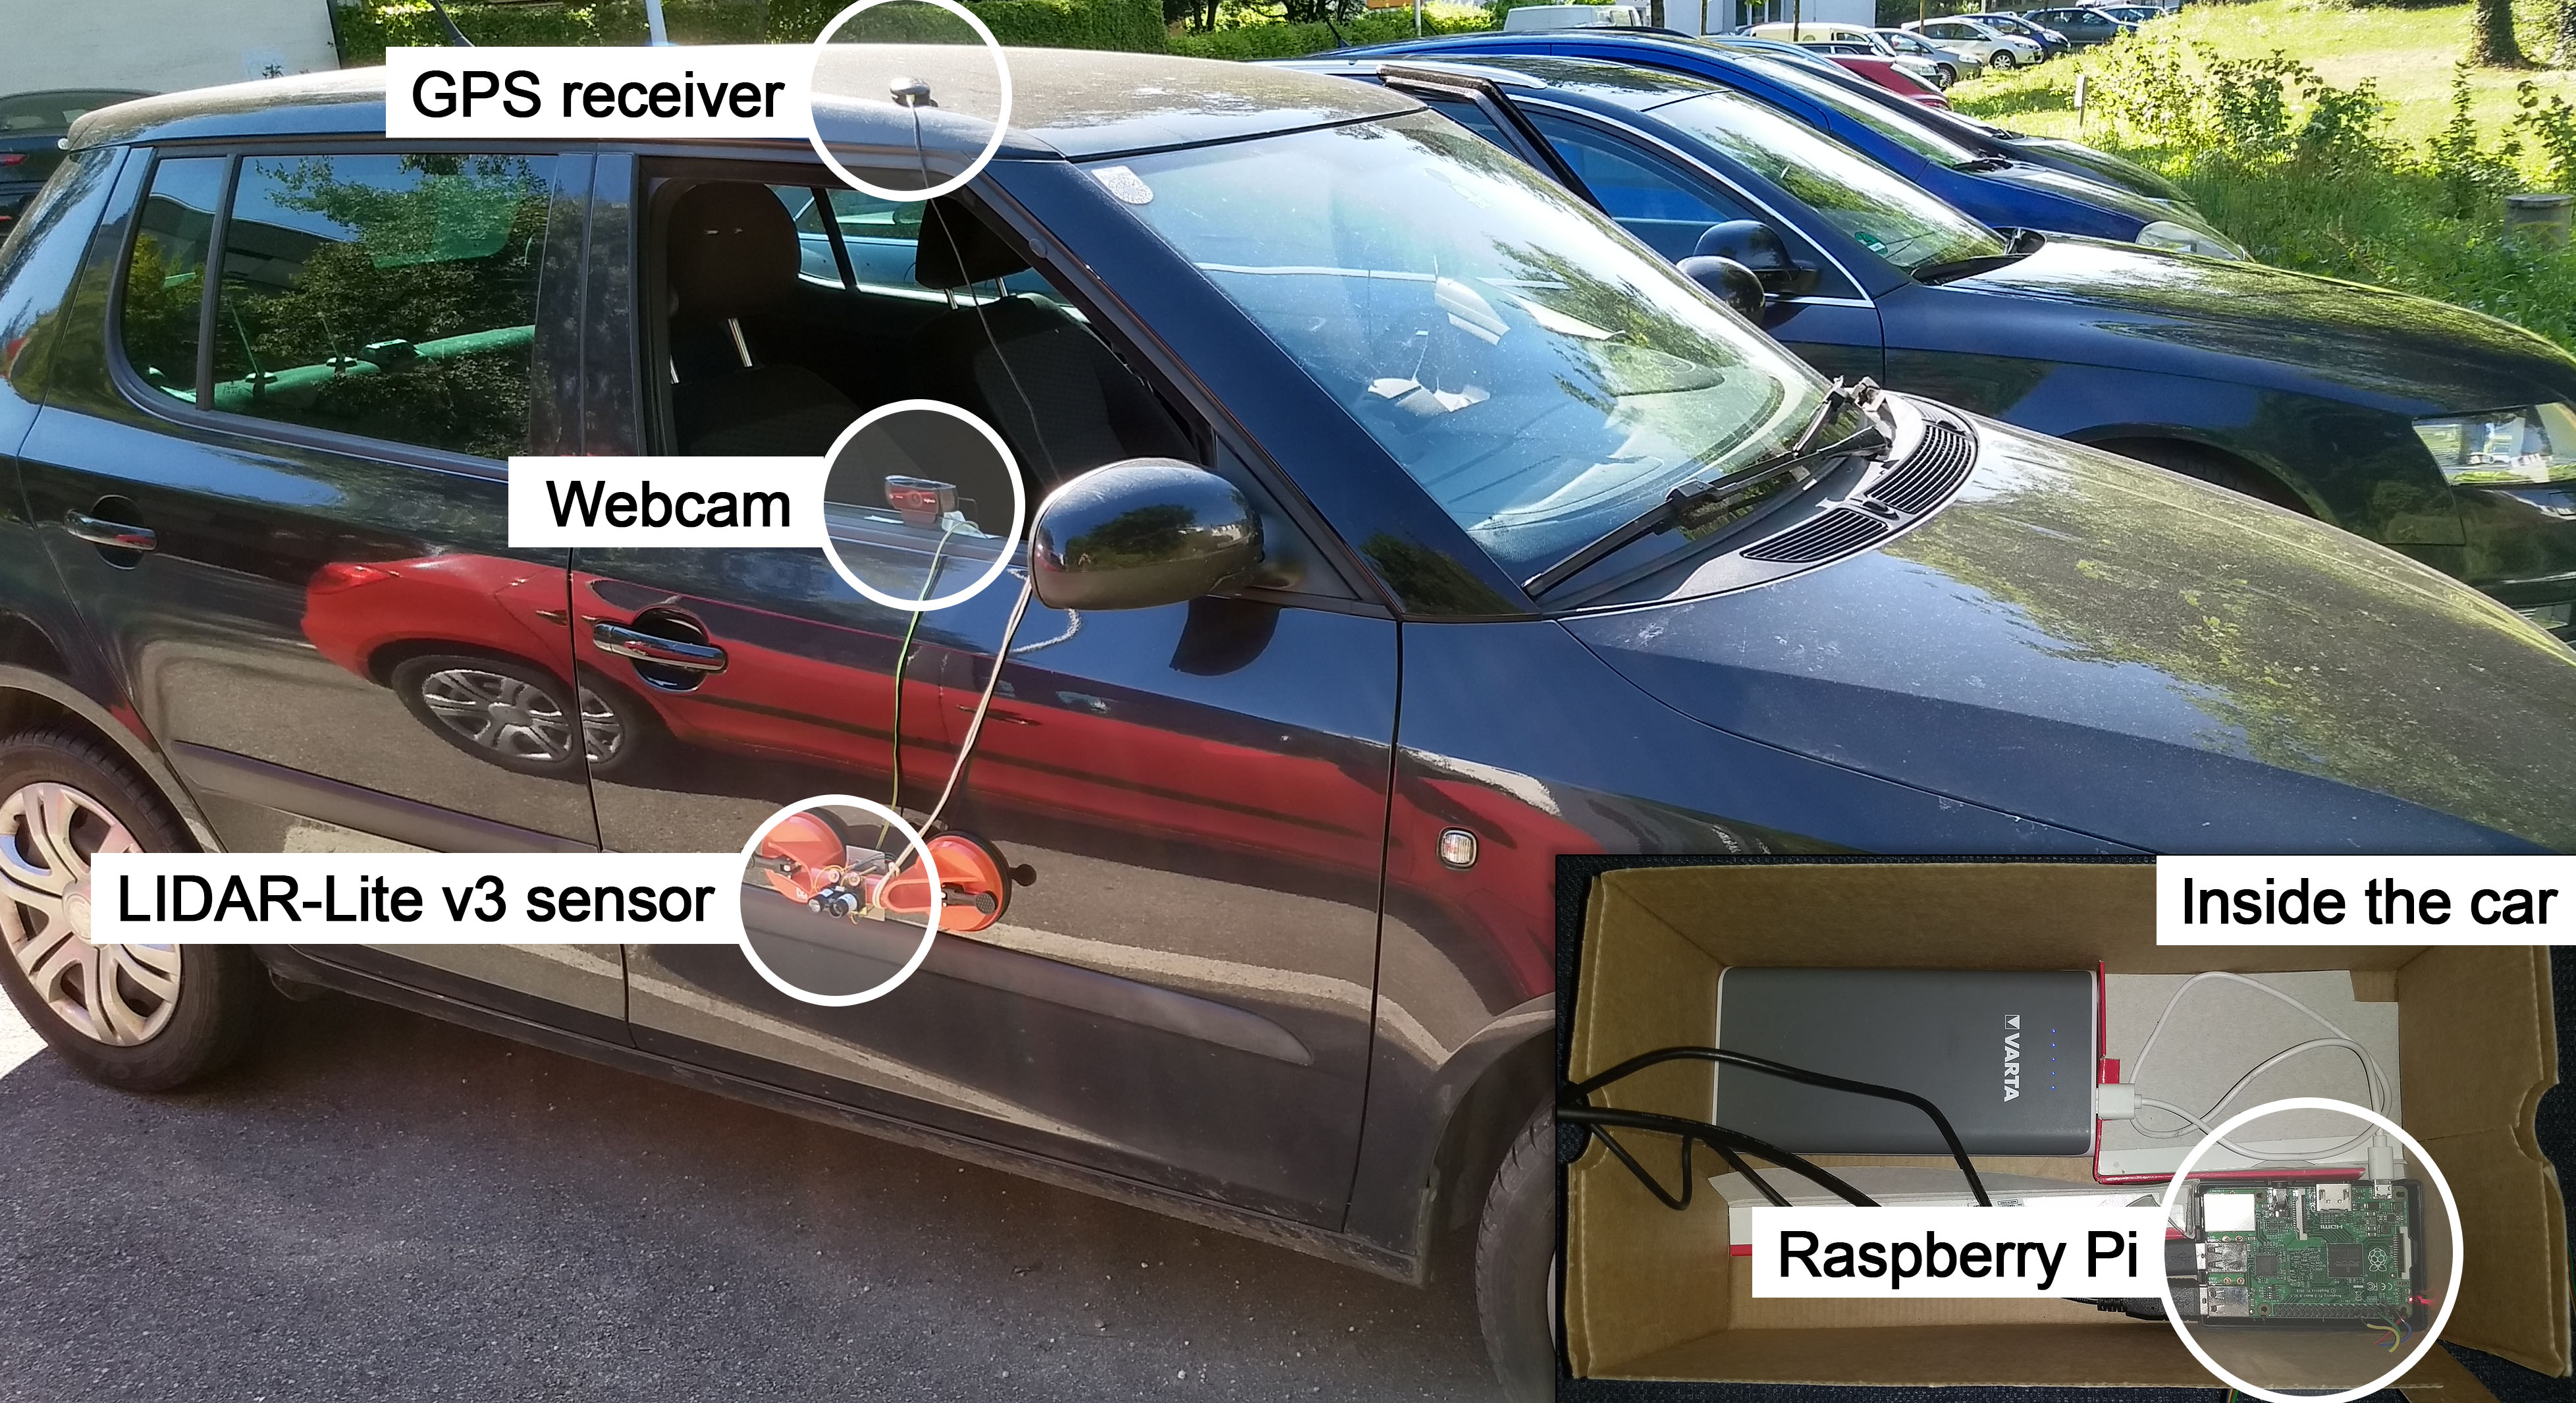
\includegraphics[width=\textwidth]{img/car.jpg}
	\caption{Prototype of the sensing car, which is composed of a LIDAR Lite v3 optical distance sensor, a GPS receiver, a camera for ground truth collection and a Raspberry Pi as processing device}
	\label{fig:sensing_car}
\end{figure}


\section{Experiment description and data collection}
\label{sec:experiment_description_data_collection}
- Description of experiments (scenarios we are interested in: parking car, etc.)
- Data set derived (raw data, size, etc.)
- Map data and camera ground truth data

\section{Data processing}
\label{sec:data_processing}
- Preprocessing, feature definition ...
- Traditional ML Algorithms (incl. a short description of each algorithm and configuration options)
- Deep Learning

\section{Experimental results}
- Results of the different ML approaches, important features, difficult cases, etc.
- Comparison of traditional ML and Deep Learning (cf. our demo)